% Writing pack for the co-author. Compile from the REPOSITORY ROOT:
%   tectonic -X compile WRITING_PACK.tex
% Fonts are macOS system faces. On another platform, swap the three
% \set*font lines below for any serif / sans / mono you have installed.
\documentclass[11pt]{article}

\usepackage{fontspec}
\setmainfont{Charter}[Numbers=OldStyle]
\setsansfont{Avenir Next}[Scale=0.95]
\setmonofont{Menlo}[Scale=0.83]

\usepackage[letterpaper,top=0.95in,bottom=1in,left=1.05in,right=1.05in]{geometry}
\usepackage[table]{xcolor}
\usepackage{booktabs}
\usepackage{tabularx}
\usepackage{array}
\usepackage{titlesec}
\usepackage{enumitem}
\usepackage{fancyhdr}
\usepackage{graphicx}
\usepackage{ragged2e}
\usepackage[hidelinks]{hyperref}

\definecolor{accent}{RGB}{14,90,97}
\definecolor{brick}{RGB}{143,58,44}
\definecolor{ink}{RGB}{20,24,28}
\definecolor{muted}{RGB}{104,116,124}
\definecolor{rule}{RGB}{214,220,223}
\definecolor{wash}{RGB}{240,245,245}
\definecolor{washwarn}{RGB}{249,238,235}

\color{ink}

\titleformat{\section}{\sffamily\bfseries\large\color{accent}}{\thesection}{0.7em}{}
\titlespacing*{\section}{0pt}{20pt}{7pt}
\titleformat{\subsection}{\sffamily\bfseries\normalsize\color{ink}}{\thesubsection}{0.6em}{}
\titlespacing*{\subsection}{0pt}{14pt}{4pt}

\pagestyle{fancy}
\fancyhf{}
\renewcommand{\headrulewidth}{0.3pt}
\renewcommand{\footrulewidth}{0pt}
\fancyhead[L]{\sffamily\footnotesize\color{muted}NHANES cognition paper \textbullet\ writing pack}
\fancyhead[R]{\sffamily\footnotesize\color{muted}\thepage}

\setlength{\parindent}{0pt}
\setlength{\parskip}{7pt}
\renewcommand{\arraystretch}{1.25}

\newcommand{\lbl}[1]{{\sffamily\footnotesize\bfseries\color{muted}\MakeUppercase{#1}}}
\newcommand{\num}[1]{{\ttfamily #1}}
\newcommand{\hdF}[1]{\multicolumn{1}{@{}l}{\lbl{#1}}}
\newcommand{\hdM}[1]{\multicolumn{1}{l}{\lbl{#1}}}

\newenvironment{callout}[1]{%
  \par\medskip
  {\color{accent}\hrule height 1.1pt}
  \vspace{7pt}
  \lbl{#1}\par\vspace{2pt}
  \begingroup\leftskip=1.15em \rightskip=0.7em
}{%
  \par\endgroup
  \vspace{7pt}
  {\color{rule}\hrule height 0.5pt}
  \par\medskip
}

\begin{document}

\begin{center}
{\sffamily\footnotesize\color{muted}\MakeUppercase{Writing pack \textbullet\ prepared 3 September 2026}}\\[10pt]
{\LARGE\bfseries Everything you need to start writing}\\[8pt]
{\large\color{muted}Predictive value of nutritional and toxic-metal biomarkers\\for cognitive performance in older adults}\\[10pt]
{\sffamily\footnotesize\color{muted}NHANES 2011--2014 \textbullet\ \texttt{github.com/NeilP211/nhanes-ieee} (private)}
\end{center}

\vspace{4pt}
{\color{rule}\hrule height 0.6pt}
\vspace{10pt}

Analysis is finished and locked. Methods and Results are drafted in manuscript prose. What follows is every number, every framing decision, and every defence you need, in one place. Nothing here is new analysis; every figure traces to a file in \num{output/tables/}.

\section*{Where things actually stand}
\addcontentsline{toc}{section}{Where things actually stand}

\begin{tabularx}{\textwidth}{@{}p{4.3cm} X@{}}
\toprule
\hdF{Done and locked} & Variable list, dated pre-registration, cohort, outcome, all modelling, evaluation, interpretation, six sensitivity analyses, five figures, TRIPOD+AI checklist, Methods and Results prose. \\
\hdF{Cannot move} & Every number below. The pre-registration is dated before modelling; changing an analysis now voids the pre-specification claim, which is the paper's main asset. \\
\hdF{Open, gates writing} & Venue. See below. \\
\hdF{Open, Shreyan's} & Introduction and Discussion, per brief section 12. \\
\hdF{Open, admin} & \textbf{The pre-registration is not countersigned.} Section 10 of \num{PREREGISTRATION.md} still reads ``pending countersign'' for the clinical lead. Close this. \\
\bottomrule
\end{tabularx}

\section{The one decision that gates writing}

Your own brief already called this, in bold, in section 7:

\begin{callout}{From PROJECT\_BRIEF.md section 7}
``IEEE and nutrition journals want genuinely different papers. IEEE foregrounds the ML and treats cognition as the application; Nutrients foregrounds the nutrition and treats ML as the tool. \textbf{The introductions are not interchangeable. Pick a lane before your co-author starts drafting.}''
\end{callout}

The result landed as \textbf{Scenario C} (null on the primary axis) combined with \textbf{Scenario E} (flexible learners do not beat penalized regression). The brief's own decision rule routes ``C (any)'' to a methodological framing at Diagnostic and Prognostic Research, Journal of Clinical Epidemiology, or PLOS ONE, and says Scenario E ``weakens an IEEE framing.''

\subsection*{Recommendation: Diagnostic and Prognostic Research (BMC)}

\begin{itemize}[leftmargin=1.2em,itemsep=3pt,topsep=4pt]
\item The only venue your brief rates \textbf{Excellent}. It exists specifically for prediction-model studies, so an incremental-value null is its remit rather than a hard sell.
\item TRIPOD-native, and the completed TRIPOD+AI checklist is already sitting in \num{output/}.
\item The brief's structural argument: with a clinically focused co-author doing literature review and interpretation, the clinical route fits the team you actually have.
\end{itemize}

\textbf{The honest case for the other lane.} You did build the two things section 7 said would raise IEEE odds: a mixture-method benchmark evaluated on predictive rather than inferential criteria, and a bootstrapped rank-stability analysis. Those are real computational content, not a classifier bake-off. What you did not get is Scenario D, where ML beats logistic, which was the other lever. So IEEE Access remains arguable but is now the harder sell. IEEE EMBC is better treated as a possible parallel four-page conference submission later, subject to each venue's dual-submission policy, than as the primary target.

\textbf{What this changes if you pick DPR:} the Introduction leads with the association-versus-prediction gap as a methodological problem, not with metals toxicology. The mixture benchmark becomes supporting evidence rather than the headline contribution. Nothing in Methods or Results changes.

\section{The headline, stated three ways}

\textbf{One sentence.} Biomarkers that this literature reports as associated with cognition do not help identify who has low cognitive performance once you know a person's age, education and income.

\textbf{One paragraph.} Across 1,784 US adults aged 60 and over, adding five blood metals and fifteen nutritional and metabolic biomarkers to a demographics-only model changed cross-validated discrimination by \num{-0.0019} AUC (95\% CI \num{-0.0108} to \num{0.0071}). The interval's upper bound falls below the 0.02 improvement declared meaningful in advance, so the analysis excludes a worthwhile gain rather than merely failing to detect one. The same twenty-analyte panel performed measurably worse than eight items of routine clinical history.

\textbf{The technical claim.} $\Delta$AUC(M3 $-$ M0) $=$ \num{-0.0019}, 95\% CI [\num{-0.0108}, \num{0.0071}], from 2,000 paired bootstrap resamples, stratified 10-fold cross-validation repeated five times, n $=$ 1,784, 431 events. H1 not supported, H0 retained, and the pre-specified meaningful-difference threshold excluded.

\begin{center}
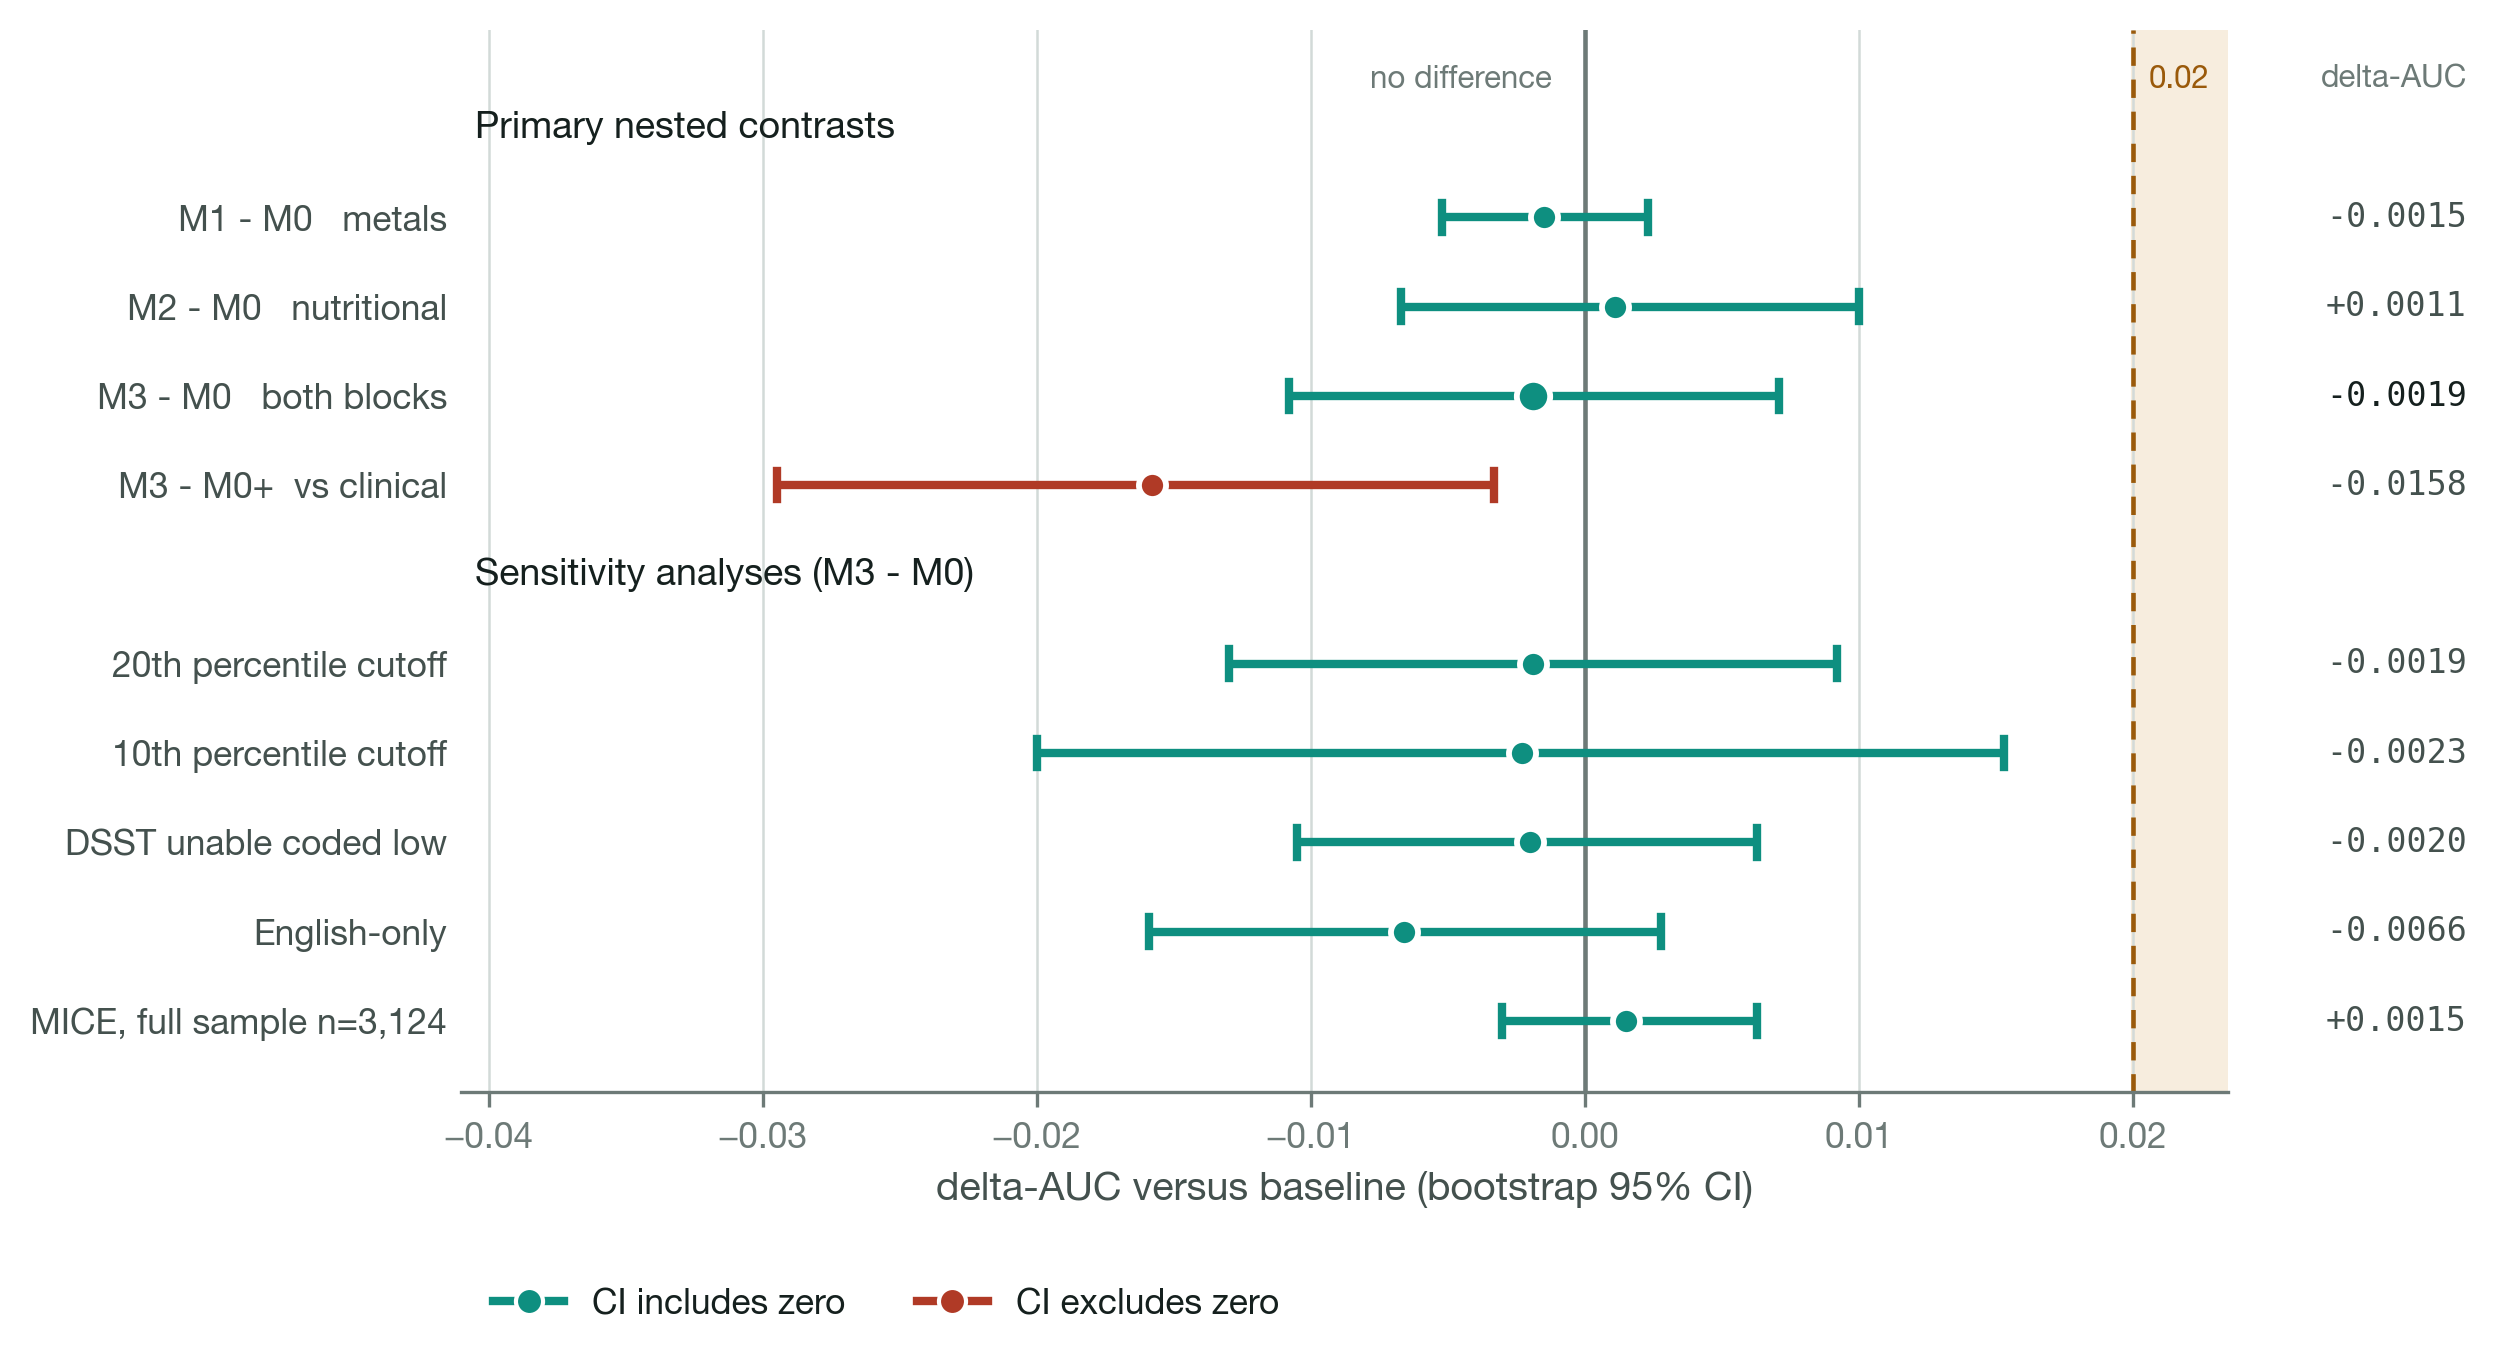
\includegraphics[width=0.93\textwidth]{output/figures/fig1_delta_auc_forest.png}
\end{center}

\section{Draft structured abstract}

Ready to edit. Every number is real. Roughly 360 words, which suits BMC-family limits.

\begin{callout}{Draft, structured}
\textbf{Background.} Multiple studies report associations between blood metals, nutritional biomarkers and cognitive performance among US adults aged 60 and over in NHANES 2011--2014. None report whether those biomarkers identify which individuals have low cognitive performance, or whether they add to information already available without a laboratory.

\textbf{Methods.} We analysed NHANES 2011--2012 and 2013--2014, restricted to examined participants aged 60 and over. Low cognitive performance was defined as the lowest quartile of a composite z-score from CERAD immediate and delayed recall, animal fluency, and the Digit Symbol Substitution Test. Four nested specifications were fixed in advance: demographics (M0); demographics plus five blood metals (M1); demographics plus fifteen nutritional and metabolic biomarkers (M2); and both blocks (M3). A pre-specified secondary baseline (M0+) added eight routinely recorded clinical covariates. Three algorithms (L2-penalized logistic regression, random forest, gradient boosting) were evaluated by stratified 10-fold cross-validation repeated five times, with all preprocessing and hyperparameter selection performed inside training folds. The pre-specified primary measure was $\Delta$AUC(M3 $-$ M0) with a 2,000-sample paired bootstrap interval; 0.02 was declared in advance as the smallest meaningful improvement. Reporting follows TRIPOD+AI.

\textbf{Results.} Of 3,124 participants with an outcome label, 1,784 had complete predictor data, of whom 431 (24.2\%) met the definition of low cognitive performance. Demographics alone reached AUC 0.788. $\Delta$AUC(M3 $-$ M0) was \num{-0.0019} (95\% CI \num{-0.0108} to \num{0.0071}), with the upper bound below the pre-specified 0.02 threshold. Neither biomarker block contributed alone. M3 performed worse than the clinical baseline M0+ ($\Delta$AUC \num{-0.0158}, 95\% CI \num{-0.0295} to \num{-0.0033}), consistently across all three algorithms. Decision-curve analysis identified no threshold probability at which the panel added net benefit. Quantile g-computation on the metal mixture achieved AUC 0.7874, no better than demographics alone. Across 200 bootstrap resamples, education, age and income-to-poverty ratio occupied the top three ranks in at least 99\% of resamples, while every biomarker moved across 15 to 20 ranks. The null persisted in all six pre-specified sensitivity analyses, including multiple imputation on the full labelled sample of 3,124 ($\Delta$AUC \num{0.0015}, 95\% CI \num{-0.0030} to \num{0.0063}).

\textbf{Conclusions.} Reported biomarker-cognition associations did not translate into individual-level predictive utility beyond age, education and income, and a twenty-analyte laboratory panel was outperformed by eight items of routine clinical history. Because the interval excludes the improvement specified in advance as meaningful, this is a precise null rather than an inconclusive one.
\end{callout}

\section{Title options}

\begin{enumerate}[leftmargin=1.4em,itemsep=6pt,topsep=4pt]
\item \textbf{Reported biomarker-cognition associations do not translate into predictive utility: a pre-registered analysis of NHANES 2011--2014.}\\
{\small\color{muted}The brief's own Scenario C suggestion. Leads with the methodological claim. Best fit for DPR or JCE.}
\item \textbf{A twenty-analyte biomarker panel adds nothing beyond age, education and income for identifying low cognitive performance in older adults.}\\
{\small\color{muted}Leads with the concrete finding rather than the abstraction. More quotable, slightly more combative.}
\item \textbf{Association is not prediction: incremental value of nutritional and toxic-metal biomarkers for low cognitive performance, NHANES 2011--2014.}\\
{\small\color{muted}Colon construction is conventional for methods venues. ``Association is not prediction'' is the sentence a reviewer remembers.}
\end{enumerate}

Do not use ``cognitive impairment'' in any title. See the language rules.

\section{Every number you can quote}

\subsection{Primary contrasts, L2-penalized logistic}

\begin{tabularx}{\textwidth}{@{}X r l c c@{}}
\toprule
\hdF{Contrast} & \lbl{$\Delta$AUC} & \lbl{95\% CI} & \lbl{Excl. 0} & \lbl{$>$ 0.02} \\
\midrule
M1 $-$ M0, metals block & \num{-0.0015} & [\num{-0.0052}, \num{0.0023}] & no & no \\
M2 $-$ M0, nutritional block & \num{0.0011} & [\num{-0.0067}, \num{0.0100}] & no & no \\
\textbf{M3 $-$ M0, both blocks} & \textbf{\num{-0.0019}} & \textbf{[\num{-0.0108}, \num{0.0071}]} & \textbf{no} & \textbf{no} \\
M3 $-$ M0+, vs clinical baseline & \textcolor{brick}{\num{-0.0158}} & \textcolor{brick}{[\num{-0.0295}, \num{-0.0033}]} & \textcolor{brick}{\textbf{yes}} & no \\
\bottomrule
\end{tabularx}

H3 is not supported: neither block contributes, so non-redundancy between blocks does not arise.

\subsection{M3 versus the clinical baseline, all three algorithms}

\begin{tabularx}{\textwidth}{@{}X r l@{}}
\toprule
\hdF{Algorithm} & \lbl{$\Delta$AUC (M3 $-$ M0+)} & \lbl{95\% CI} \\
\midrule
L2-penalized logistic & \num{-0.0158} & [\num{-0.0295}, \num{-0.0033}] \\
Random forest & \num{-0.0197} & [\num{-0.0338}, \num{-0.0055}] \\
Gradient boosting (XGBoost) & \num{-0.0230} & [\num{-0.0385}, \num{-0.0063}] \\
\bottomrule
\end{tabularx}

M0+ is demographics plus BMI, smoking, alcohol, PHQ-9 depression score, and self-reported stroke, diabetes, hypertension and high cholesterol. Eight questions, no blood draw.

\subsection{Discrimination and calibration}

Mean out-of-fold across five repeats of stratified 10-fold CV, n $=$ 1,784.

\begin{tabularx}{\textwidth}{@{}l X r r r r r@{}}
\toprule
\lbl{Spec} & \hdM{Algorithm} & \lbl{AUC} & \lbl{AUPRC} & \lbl{Brier} & \lbl{Cal. slope} & \lbl{Cal. int.} \\
\midrule
M0 & logistic & 0.7884 & 0.5471 & 0.1459 & 1.088 & 0.001 \\
M0 & random forest & 0.7843 & 0.5363 & 0.1466 & 1.148 & 0.004 \\
M0 & xgboost & 0.7845 & 0.5399 & 0.1470 & 0.898 & 0.004 \\
M1 & logistic & 0.7868 & 0.5456 & 0.1465 & 1.069 & 0.002 \\
M2 & logistic & 0.7895 & 0.5420 & 0.1461 & 1.026 & 0.002 \\
M3 & logistic & 0.7865 & 0.5392 & 0.1470 & 1.004 & 0.002 \\
M3 & random forest & 0.7806 & 0.5384 & 0.1501 & 1.410 & \num{-0.012} \\
M3 & xgboost & 0.7779 & 0.5201 & 0.1497 & 0.904 & 0.024 \\
\textbf{M0+} & \textbf{logistic} & \textbf{0.8023} & \textbf{0.5618} & \textbf{0.1423} & \textbf{1.042} & \textbf{0.003} \\
\bottomrule
\end{tabularx}

Every model discriminates reasonably (AUC 0.78 to 0.80) and essentially all of it comes from age, education and income. Logistic is best calibrated as well as best discriminating: random forest is over-dispersed (slope up to 1.41), XGBoost slightly under (about 0.90).

\subsection{H2: nonlinear learners do not win}

\begin{tabularx}{\textwidth}{@{}X r l@{}}
\toprule
\hdF{Contrast on M3} & \lbl{$\Delta$AUC} & \lbl{95\% CI} \\
\midrule
Random forest $-$ logistic & \num{-0.0059} & [\num{-0.0175}, \num{0.0060}] \\
XGBoost $-$ logistic & \num{-0.0086} & [\num{-0.0187}, \num{0.0007}] \\
\bottomrule
\end{tabularx}

The rationale behind H2 also fails on its own terms. Partial dependence for selenium and manganese, the two exposures expected to show U-shaped exposure-response, shows no such shape: the extremum sits near an end of the range and the total swing in predicted probability is about 0.05 for each.

\subsection{Clinical utility}

Net benefit for M3 against M0 across threshold probabilities from 0.05 to 0.60.

\begin{itemize}[leftmargin=1.2em,itemsep=2pt,topsep=3pt]
\item M3 exceeds M0 at \textbf{21 of 56} thresholds, indistinguishable from chance.
\item Maximum net-benefit gain of M3 over M0 is \textbf{0.0059}, negligible.
\item M0+ exceeds M0 at \textbf{52 of 56} thresholds.
\end{itemize}

There is no plausible decision threshold at which adding the panel would change a decision. The clinical-utility claim is null on its own terms, not only on discrimination.

\subsection{Mixture-method benchmark}

Quantile g-computation, reimplemented in Python with training-fold quantile cutpoints so it fits inside the CV loop without leakage.

\begin{tabularx}{\textwidth}{@{}X r@{}}
\toprule
\hdF{Model} & \lbl{Cross-validated AUC} \\
\midrule
Demographics only (M0) & 0.7884 \\
Quantile g-computation, metals mixture + demographics & 0.7874 \\
M1, metals as individual features + demographics & 0.7868 \\
\bottomrule
\end{tabularx}

Joint mixture effect $\psi = $ \num{-0.1162} in log-odds per simultaneous one-quartile increase. Component weights: cadmium 0.820 and lead 0.180 positive; mercury \num{-0.376}, manganese \num{-0.365}, selenium \num{-0.260} negative.

BKMR was excluded in advance (convergence fragility for binary outcomes, and cost inside 50 folds). WQS was deferred because its package partitions data internally in a way that conflicts with external cross-validation, and with no predictive signal in the metals block there is no basis for adding it.

\subsection{Feature importance and rank stability}

Bootstrapped SHAP over 200 resamples of the M3 XGBoost model.

\begin{tabularx}{\textwidth}{@{}X r c r@{}}
\toprule
\hdF{Feature} & \lbl{Median rank} & \lbl{95\% rank interval} & \lbl{In top 5} \\
\midrule
Education (\num{DMDEDUC2}) & 1 & 1 to 2 & 100\% \\
Age (\num{RIDAGEYR}) & 2 & 1 to 2 & 100\% \\
Income to poverty (\num{INDFMPIR}) & 3 & 3 to 5 & 99\% \\
Neutrophil-to-lymphocyte ratio & 5 & 3 to 19 & 51\% \\
eGFR & 7 & 4 to 19 & 34\% \\
HDL cholesterol & 7 & 4 to 19 & 35\% \\
Vitamin B12 & 8 & 4 to 19 & 25\% \\
Cadmium & 14 & 5 to 24 & 4.5\% \\
Selenium & 14 & 6 to 23 & 2.5\% \\
\bottomrule
\end{tabularx}

The three demographics are rank-stable to the point of determinism; every biomarker swings across a 15 to 20 rank interval between resamples. That instability is itself a result, and a direct methodological caution for a literature that reports single-run rankings without resampling.

\subsection{Sensitivity analyses, all six pre-specified}

\begin{tabularx}{\textwidth}{@{}X r r l@{}}
\toprule
\hdF{Analysis} & \lbl{n} & \lbl{$\Delta$AUC} & \lbl{95\% CI} \\
\midrule
Primary (reference) & 1,784 & \num{-0.0020} & [\num{-0.0103}, \num{0.0066}] \\
Cutoff at 20th percentile & 1,784 & \num{-0.0019} & [\num{-0.0130}, \num{0.0092}] \\
Cutoff at 10th percentile & 1,784 & \num{-0.0023} & [\num{-0.0200}, \num{0.0153}] \\
DSST ``unable'' coded low (25 recoded) & 1,784 & \num{-0.0020} & [\num{-0.0105}, \num{0.0063}] \\
English-only administration & 1,575 & \num{-0.0066} & [\num{-0.0159}, \num{0.0028}] \\
\textbf{MICE on full labelled sample} & \textbf{3,124} & \textbf{\num{0.0015}} & \textbf{[\num{-0.0030}, \num{0.0063}]} \\
\bottomrule
\end{tabularx}

\textbf{Leave-one-block-out.} Dropping metals: \num{-0.0028} [\num{-0.0051}, \num{-0.0004}], CI excludes zero, so removing the metals block slightly \emph{improves} discrimination. Dropping nutritional: \num{-0.0002} [\num{-0.0081}, \num{0.0078}]. The metals contribute noise rather than signal.

\textbf{Continuous outcome.} Cross-validated $R^2$ for the composite z-score is 0.3825 for M0 and 0.3908 for M3, a gain of 0.0083. This is the only result pointing in the positive direction: about 0.8\% additional variance explained, which does not translate into discrimination for the binary outcome.

\subsection{Participants, for the flow diagram}

\begin{tabularx}{\textwidth}{@{}X r@{}}
\toprule
\hdF{Stage} & \lbl{n} \\
\midrule
Participants in both cycles & 19,931 \\
Aged 60 or older & 3,632 \\
Completed the examination visit & 3,472 \\
At least 3 of 4 cognitive scores, outcome label assigned & 3,124 \\
\textbf{Complete predictors and covariates, analytic sample} & \textbf{1,784} \\
\quad of whom met the low cognitive performance definition & 431 (24.2\%) \\
\bottomrule
\end{tabularx}

Weighted population represented: 59.7 million. The 2013--2014 cycle contributed 661 against 1,123 from 2011--2012, because blood metals in that cycle were measured in a one-half random subsample rather than in all examined participants. Excluded participants were slightly older (mean 70.1 against 69.4 years) and slightly more likely to meet the outcome definition (26.2\% against 24.1\%), all differences under three percentage points.

Outcome internal consistency: Cronbach alpha 0.795. CERAD immediate to delayed recall correlation 0.743; correlations among the three instruments 0.40 to 0.51.

\section{Language rules, non-negotiable}

These held throughout Methods and Results. Breaking them in the Introduction or Discussion creates an inconsistency a reviewer will find.

\begin{enumerate}[leftmargin=1.4em,itemsep=5pt,topsep=4pt]
\item \textbf{The outcome is ``low cognitive performance'', never ``cognitive impairment''.} NHANES contains no clinical diagnosis. This is not a stylistic preference; claiming impairment claims a diagnosis you do not have.
\item \textbf{No causal verbs anywhere.} The design is cross-sectional. Not ``leads to'', ``causes'', ``improves'', ``protects against'', ``reduces risk of''. Associations and predictions only.
\item \textbf{Say what the null is about.} Nothing here shows any biomarker is unrelated to cognition. The published associations may all be correct. The finding is that they do not translate into identifying \emph{which individuals} have low cognitive performance once age, education and income are known. That distinction is the paper.
\item \textbf{Phrase the precision deliberately.} ``The interval excludes an improvement of the magnitude specified in advance as meaningful'' is a much stronger sentence than ``the difference was not statistically significant''. It is available only because the 0.02 threshold was fixed before modelling. Do not weaken it into ordinary non-significance language.
\item \textbf{Every result states whether it is an association claim or a prediction claim.} Survey weights (\num{WTMEC2YR} halved, \num{SDMVSTRA}, \num{SDMVPSU}) are used for association claims; unweighted machine learning is used for prediction claims. Say which, each time. Expect a reviewer to ask why the prediction models are unweighted; the answer is in pre-registration section 8 and should appear in the paper.
\end{enumerate}

\section{Introduction skeleton}

\subsection*{The gap, with evidence}

Published work on this exact population and cycle range. Every one reports coefficients or odds ratios; not one reports discrimination, calibration, or cross-validation.

\begin{tabularx}{\textwidth}{@{}X r X c@{}}
\toprule
\hdF{Study} & \lbl{n} & \hdM{Method} & \lbl{Predictive metrics} \\
\midrule
Blood metals and cognition, 60+ & 1,460 & Linear regression, RCS & None \\
Iron plus 5 metals, low cognition & 2,002 & Weighted logistic & None \\
Trace elements plus DII & 1,726 & GLM, BKMR, WQS, qg-comp & None \\
Joint metal exposure & 811 & Mixture models & None \\
Sex-specific metal mixtures & n/r & Mixture models & None \\
Metals by diet quality & 1,777 & Quantile g-computation & None \\
Cadmium by omega-6 intake & 1,918 & Logistic & None \\
\bottomrule
\end{tabularx}

Shreyan will want to replace these descriptors with the actual citations during the literature review. The structural point is the last column.

\subsection*{The argument, in order}

\begin{enumerate}[leftmargin=1.4em,itemsep=4pt,topsep=4pt]
\item The literature on this population is saturated on association and empty on prediction. That asymmetry is the opportunity.
\item This is a different question, not a different variable. Adding exposure number 48 to a saturated association literature is incremental; asking whether any of it predicts is categorical. A reviewer cannot say this has been done, because it has not.
\item The gap between statistical association and predictive utility is a recognised methodological problem. Demonstrating it concretely in a heavily mined dataset has value beyond this exposure-outcome pair.
\item Calibration, decision-curve analysis and TRIPOD+AI reporting are what prediction-model reviewers expect, and none of the comparison papers provide them.
\end{enumerate}

\subsection*{Honest limits of the novelty claim, state these explicitly}

The data are not novel: NHANES 2011--2014 is heavily mined. The algorithms are not novel: penalized logistic, random forest and XGBoost are standard. The contribution is the question, the evaluation framework, and the reporting standard. Say so plainly. Overclaiming novelty is the fastest route to a hostile review, and the brief flags exactly this.

\section{Discussion skeleton}

\subsection*{Three things that lift this above a bare null}

\begin{enumerate}[leftmargin=1.4em,itemsep=5pt,topsep=4pt]
\item \textbf{The null is precise, not underpowered.} The confidence interval excludes the pre-specified meaningful difference. This is the strongest sentence available in the paper.
\item \textbf{The panel is significantly worse than a questionnaire.} Twenty analytes outperformed by eight items of routine clinical history, consistently across three algorithms, with intervals excluding zero. This converts an absence of evidence into a concrete statement about what actually carries information. It is the most quotable result in the paper.
\item \textbf{The field's preferred method fares no better.} Quantile g-computation, evaluated on predictive rather than inferential criteria, matched neither demographics nor the same metals as ordinary features. And single-run SHAP rankings over correlated biomarkers do not reproduce across resamples, which is a direct caution to a literature that reports them routinely.
\end{enumerate}

\subsection*{Limitations to state plainly}

\begin{itemize}[leftmargin=1.2em,itemsep=3pt,topsep=4pt]
\item The design is cross-sectional.
\item The complete-case restriction is mildly non-random, though the dominant exclusion mechanism is a random subsample by design.
\item Age is top-coded at 80, compressing its range.
\item There is no external validation cohort.
\item No subgroup fairness audit was pre-specified.
\item Serum copper and zinc were excluded because that assay was run on a one-third subsample.
\item The outcome is defined against pooled-sample quantiles, so a participant's label depends on the whole sample distribution. This was pre-specified and is a property of a relative outcome definition, but it should be stated.
\end{itemize}

\subsection*{What the paper does not claim}

That any biomarker is unrelated to cognition. That anyone should stop measuring these analytes for other clinical purposes. That the published associations are wrong. Anticipate all three misreadings and foreclose them in the Discussion.

\section{Reviewer objections, and the answers you already have}

\begin{tabularx}{\textwidth}{@{}p{5.2cm} X@{}}
\toprule
\hdF{Objection} & \hdM{Answer already in the analysis} \\
\midrule
``Your complete-case sample created the null.'' & MICE on the full labelled sample of 3,124, imputed inside folds, gives \num{0.0015} [\num{-0.0030}, \num{0.0063}]. That is the \emph{tightest} interval of any analysis and still null. Pre-empt this in the Results. \\
``You were underpowered.'' & The CI upper bound of \num{0.0071} lies below the 0.02 threshold fixed before modelling. Precision, not absence of power. \\
``The literature uses mixture models, you used ML.'' & Quantile g-computation reimplemented inside the CV loop with training-fold cutpoints: AUC 0.7874 against 0.7884 for demographics alone. No advantage. \\
``Nonlinearity would show a signal.'' & Random forest and XGBoost fitted to every specification; both tie or lose. Partial dependence shows no U-shape for selenium or manganese. \\
``Optimism or leakage.'' & All preprocessing and tuning inside training folds, plus an automated audit that refits a fold and asserts the scaler matches training-fold statistics, not full-sample. It fails the run rather than warning, and it passed. \\
``Your quartile cutoff is arbitrary.'' & Cutoffs at the 10th and 20th percentiles, plus the continuous composite as a regression outcome. All null. \\
``Why unweighted models?'' & Pre-registration section 8: weights for association claims, unweighted ML for prediction claims. State the rationale in the paper rather than leaving it to be asked. \\
``Language of administration confounds cognition scores.'' & English-only restriction, n $=$ 1,575: \num{-0.0066} [\num{-0.0159}, \num{0.0028}]. \\
\bottomrule
\end{tabularx}

\section{What exists, and where}

\begin{tabularx}{\textwidth}{@{}p{5.6cm} X@{}}
\toprule
\hdF{Asset} & \hdM{Contents} \\
\midrule
\num{MANUSCRIPT\_DRAFT.md} & Methods and Results in final prose, plus a ``Notes for the co-author'' block at the end. \\
\num{PREREGISTRATION.md} & Hypotheses and analysis plan, dated before modelling. Countersign still pending. \\
\num{VARIABLE\_LOCK.md} & Locked variable list with dated amendments. \\
\num{output/TRIPOD\_AI\_checklist.md} & Completed, ready as a supplementary file. \\
\num{output/tables/} & Eight result tables as CSV and markdown. \\
\num{output/results\_review.html} & Full results review in one page. \\
Figure 1 & Forest plot of $\Delta$AUC contrasts. \\
Figure 2 & Calibration, out-of-fold, decile bins. \\
Figure 3 & Decision-curve analysis. \\
Figure 4 & Rank stability across 200 bootstrap resamples. \\
Figure 5 & Partial dependence, no U-shape for either essential metal. \\
\bottomrule
\end{tabularx}

All five figures exist at 300 dpi PNG and as vector PDF. The whole pipeline reproduces in under an hour on one machine with no GPU; \num{00b\_download.py} rebuilds the raw data from CDC URLs.

\vspace{14pt}
{\color{rule}\hrule height 0.6pt}
\vspace{6pt}
\begin{sloppypar}\RaggedRight
{\sffamily\footnotesize\color{muted}Sources: \num{output/tables/07\_results\_summary.md}, \num{04\_delta\_auc.csv}, \num{04\_performance.csv}, \num{05\_qgcomp.csv}, \num{06\_sensitivity.csv}, \num{MANUSCRIPT\_DRAFT.md}, \num{PROJECT\_BRIEF.md} sections 2, 6 and 7, \num{PREREGISTRATION.md} sections 8 and 10. No number in this document was computed here.}
\end{sloppypar}

\end{document}
